\documentclass[final]{svjour2}
\usepackage{graphicx}
\usepackage{rotating}
\usepackage{amssymb}
\usepackage{wrapfig}
\usepackage{subfig}
\usepackage{amsmath}
\usepackage{mathptmx}
\usepackage[numbers]{natbib}
\usepackage[table]{xcolor}
\usepackage{tabularx}
\usepackage{multirow}
\usepackage{booktabs}
\usepackage{threeparttable}
\usepackage{epstopdf}

\providecommand{\e}[1]{\ensuremath{\times 10^{#1}}}
\renewcommand{\thefootnote}{\alph{footnote}}

\providecommand{\p}[1]{\phantom{#1}}

%\usepackage[nofighead,nomarkers]{endfloat}
\makeatletter
\journalname{Journal of Low Temperature Physics}
%%%%%%%%%%%%%%%%%%%%%%%%%%%%%% Textclass specific LaTeX commands.


%%%%%%%%%%%%%%%%%%%%%%%%%%%%%% User specified LaTeX commands.
\bibpunct{}{}{,}{s}{}{,}

\begin{document}

\newcommand{\hdblarrow}{H\makebox[0.9ex][l]{$\downdownarrows$}-}
\title{Sub-Kelvin Thermal Conductivity and Radioactivity of Some Useful Materials in Low Background Cryogenic Experiments}

\author{N. Kellaris \and M. Daal \and M. Epland \and M. Pepin \and O. Kamaev \and P. Cushman \and E. Kramer \and B. Sadoulet \and N. Mirabolfathi \and S. Golwala \and M. Runyan}

\institute{CDMS Experiment \\ Department of Physics, University of California, Berkeley\\ Berkeley, CA 94720, USA\\
\email{nicholaskellaris@berkeley.edu}}

\date{XX.XX.20XX}

\maketitle


\begin{abstract}
     We present measurements of the thermal conductivity between 0.05K to 1K, and radioactive contamination levels, for some thermally isolating materials. TIMET Ti 15-3-3-3, Mersen grade 2020 graphite, Vespel SP-1, Vespel SP-22, Vespel SCP-5000, Vespel SCP-5050, Graphlite CFRP, and a Kapton/epoxy composite are all investigated. Thermal conductivities were measured using a single-heater longitudinal heat flow method. Material radioactivity was determined for the materials at a low background counting facility using a high-purity gamma detector and GEANT4 Monte Carlo simulations.


\keywords{Ti 15-3-3-3, Vespel, Graphite, Kapton, Thermal Conductivity, Radioactivity}

\end{abstract}

\section{Introduction}
Low temperature detector experiments often require materials with low thermal conductivity and -- in the case of low background experiments such as dark matter and double-beta decay -- low radioactivity; however, sub-Kelvin thermal conductivity and low-level radioactivity data are seldom available in the literature. Therefore, we present thermal conductivity and radioactivity data for materials which were investigated for use in the CDMS SNOLab Experiment in the hopes that they may prove useful for other cryogenic experiments. Not all materials presented here were tested for both thermal conductivity and radioactivity.

\section{Materials Tested}
Four types of DuPont Vespel polyimide were tested: SP-1, SP-22, SCP-5000, and SCP-5050. SP-1 is unfilled polyimide, while SP-22 is filled polyimide base (SP-1) with 40\% graphite by weight. SCP-5000 and SCP-5050 are the newer analogs of SP-1 and SP-22 respectively; according to DuPont, they have improved mechanical properties over the SP series. All were purchased from Curbell Plastics.

Two grades of graphite were tested. Mersen grade 2020 is anisotropic nuclear grade graphite with grain sizes of 15$\mu$m and a porosity of 9\%. Thermal conductivity was measured perpendicular to grain orientation. POCO AXM-5Q is isotropic (5$\mu$m grain) industrial grade graphite with a porosity of 23\%.

We tested TIMET Ti 15-3-3-3, a meta-stable beta titanium alloy with composition 76Ti-15V-3Al-3Cr-3Sn by weight, and a superconducting T$_c$ at 3.89K\cite{Wikus2010}. The sample was a 0.00084 inch thick foil, rolled by Arnold Magnetic Technologies from solution-treated strip, with no annealing after rolling.

A pultruded carbon-fiber composite made by Avia Sport Composites -- called Graphlite -- was tested. This is a unidirectional material with fibers nearly uniformly oriented along the pultrusion axis. Thermal conductivity was measured for a 0.156 inch diameter rod of standard modulus material, parallel to the fiber axis.

The last material measured was a Kapton-epoxy coverlay film called Nikaflex CISV2525. The sample was a 0.001 inch cured epoxy bonding sheet -- from Hanwhaflex, product code HFB-E250YG -- on a 0.001 inch sheet of Kapton 100V.  Thermal conductivity was measured parallel to the sheet.

\section{Radioactivity of Samples}
The radioactive contamination of our samples was determined for five long-lived radioisotopes: $^{238}$U, $^{232}$Th, $^{60}$Co, $^{40}$K, and $^{137}$Cs. Measurements were performed in the Soudan Underground Laboratory using "Gopher" -- a 2.075 kg high-purity Ge gamma detector \footnotemark . Gamma events were counted for up to 30 days for each sample, then modelled using GEANT4 Monte Carlo simulations to determine contamination in each sample. A low background counting environment was provided by multiple shields: The location of the facility provides 2200 mwe of shielding from cosmic rays; the detector itself is surrounded by (innermost to outermost): 2 inches of OFHC copper, followed by 2 inches of ultra low activity (ULA) lead, and finally, 10 inches of commercial lead. Counting results are shown in Table \ref{radioactivity}.

\footnotetext{Facility contact: Priscilla Cushman. prisca@physics.umn.edu}
We find multiple materials with low contamination levels; purified AXM-5Q graphite, SP-1, SCP-5050, Ti 15-3-3-3, and Graphlite CFRP all exhibit levels which show promise for radioactivity-sensitive experiments. Particularly surprising is that the contamination for SCP-5050 is significantly less than SP-22, with up to 20 times less contamination for $^{232}$Th and 7 times less for $^{238}$U despite the two materials having very similar composition. This may be attributable to different sources for the graphite used in each grade; it may also imply variable radioactivity between batches. From the performance of SCP-5050, we can infer relatively high radiopurity for SCP-5000, as it is the base polyimide for SCP-5050. For graphite, both POCO and Mersen offer purification options. The graphite is placed in an atmosphere of chlorine gas pressurized above 15psi and heated to $\sim$2000$^o$C. The chlorine permeates the graphite and forms volatiles with impurities, allowing them to be pumped away. This process works even with bulk samples. Impurities in our graphite were reduced from 1000ppm to $<$1.4ppm for 4-inch cube samples, reducing the radioactivity in the POCO graphite by a factor of $\sim$50. Purification of grade 2020 graphite was not as effective, possibly due to its lower porosity (9\%) than AXM-5Q (23\%). While not measured for this paper, Kapton laminates are known to have a high radiopurity, which has enabled their widespread use in low background experiments.

\begin{table}[htb]
\centering
\begin{threeparttable}
\begin{tabular}{lrrrr}
\toprule
\textbf{Material} & \multicolumn{4}{c}{\quad Contamination in mBq/kg}\\
& $^{238}$U & $^{232}$Th & $^{40}$K & $^{137}$Cs \\\toprule
2020 Gr. (p) & 3.89 $\pm$ \p{0}0.60 & 79.63 $\pm$ \p{00}4.97 & 4.10 $\pm$ \p{0}1.65 & $<$ 0.20 \p{00} \\
AXM-5Q Gr. (u-p) & 117.71 $\pm$ 47.41 & 217.13 $\pm$ 138.62 & 3.59 $\pm$ \p{0}3.28 & $<$ 1.25 \p{00}\\
AXM-5Q Gr. (p) & 0.93 $\pm$ \p{0}0.26 & 4.93 $\pm$  \p{00}0.70 & 0.96 $\pm$ \p{0}1.16 & $<$ 0.28 \p{00}\\
Vespel SP-1 & $<$ 16.77 \p{00} & 5.39 $\pm$  \p{00}4.80 & $<$ 13.09 \p{00} & $<$ 2.04 \p{00}\\
Vespel SP-22 & 48.38 $\pm$ \p{0}4.83 & 211.10 $\pm$ \p{00}8.99 & 7.82 $\pm$ \p{0}6.09 &  $<$ 2.47 \p{00}\\
Vespel SCP-5050 & 7.72 $\pm$  \p{0}0.88 & 9.95 $\pm$  \p{00}2.01 & 7.26 $\pm$ \p{0}2.18 & 0.48 $\pm$ 0.26 \\
Ti 15-3-3-3 foil & 20.40 $\pm$ \p{0}3.33 & 7.97 $\pm$ \p{00}1.79 &  3.26 $\pm$ \p{0}2.14 & $<$ 0.30 \p{00}\\
Graphlite CFRP & 2.79 $\pm$ \p{0}0.89 & $<$ 2.76 \p{000}& 23.95 $\pm$ \p{0}4.96 & $<$ 0.62 \p{00}\\
\bottomrule
\end{tabular}
 \caption{{\small Activity of listed isotope for each sample. For graphite, (u-p) refers to unpurified samples, while (p) refers to samples which underwent the purification described in this section. Numbers preceded by $<$ are upper limits, and are calculated at 90\% CL. $^{60}$Co was not found in detectable amounts for any sample, so is not shown. Notice the drastic effect purification has on radioactive contaminants in graphite as shown by AXM-5Q Gr. (p) and (u-p). }}
\label{radioactivity}
\end{threeparttable}
\end{table}


\section{Experimental Configuration for Thermal Conductivity Tests}



The thermal conductivities of several materials were measured. All measurements were conducted in a $^3$He-$^4$He dilution refrigerator in the range of 0.05K - 1K, with the specific range varying depending on the material.

\begin{figure}[h]
\centering
\includegraphics[width = 0.8\textwidth]{Samples2.png}

\caption{{\small Left shows a representative test set-up for five of the seven thermal conductivity tests. Primarily two thermometers ($T_{high}$ and $T_{low}$) were used for measurements, but a third ($T_{base}$) was mounted on the fridge end to verify base temperatures. Right shows the Kapton-epoxy and Ti 15-3-3-3 samples. They were folded back onto themselves numerous times and clamped with the thermometer mounts to give a large cross-section. Middle shows the assembled sample with heater and fridge mounts at the ends and thermometer mounts in the middle. Flooding the dish-shaped heater/fridge mounts with epoxy ensures sufficient thermal contact so that the heat flow through the sample will be planar, and the gradient across the sample folds will be uniform. }}
\label{setup}
\end{figure}

Figure \ref{setup} shows a representative test set-up for the thermal conductivity tests. A single heater was used to provide power; this was a 20k$\Omega$ metal film resistor for all tests except Vespel SP-22 and Vespel SCP-5050, which used a 2k$\Omega$ resistor. We read out temperatures with three thermometers, as shown in the figure. $T_{high}$ and $T_{low}$ were Ge thermistors, while $T_{base}$ was a RuO$_2$ thermistor, all from LakeShore. A Keithley 213 was used to read out the thermometers in a 4-wire configuration and to provide power to the heater. For temperatures above 550mK, an LR-700 resistance bridge was used to read out the thermometers. $T_{high}$ and $T_{low}$ were each attached to individual copper clamp fixtures, separate from the heater/fridge mounts, to prevent any boundary resistance effects which could create a temperature measurement bias. Electrical connections used either 0.0012 inch or 0.003 inch diameter manganin wires -- depending on the sample -- all with lengths of $>$ 6 inches to thermalization with the fridge. Finally, the sample was placed within a 50mK shield which mitigated radiative heat loads on the sample.

\begin{table}[htb]
\centering
\begin{tabular}{rrr}
\toprule
\textbf{Material} & L (cm) & A (cm$^2$) \\\midrule
V. SP-22 & 3.62 & 1.27 \\
V. SCP-5000 & 2.22 & 1.30 \\
V. SCP-5050 & 3.62 & 1.30 \\
Ti 15-3-3-3 & 3.05 & 0.91 \\
Graphlite CFRP & 4.03 & 0.12 \\
2020 graphite & 1.42 & 12.97 \\
Kapton-epoxy & 3.05 & 1.17 \\
\bottomrule
\end{tabular}
\caption{{\small Length and cross-section for thermal conductivity samples. L refers to the center-to-center thermometer separation.}}
\label{dim}
\end{table}

Table \ref{dim} gives dimensions for tested samples. Samples were cylindrical rods, with the exception of the Ti 15-3-3-3 and Kapton-epoxy samples; these were strips of material folded back on itself repeatedly then clamped with the thermometer mounts, as shown in the right side of Figure \ref{setup}. Copper mounts were glued to the ends of each sample using Hardman's Double-Bubble Epoxy for the Ti 15-3-3-3, Kapton-epoxy, and grade 2020 graphite, and Stycast 1266 for all other samples. The strip samples used copper dishes at either end which were flooded with epoxy to ensure good thermal contact with the sample.

\section{Thermal Conductivity Measurement Methods}
The longitudinal heat flow method was used in all tests to measure thermal conductivity. We applied a heat load to the top of the sample and let it reach equilibrium, which established a temperature gradient along the sample; this took between 30-180 minutes depending on the sample and temperature range. Once in equilibrium, we relate power through the sample and K(T) with
\begin{equation}
P = P_{heater} + P_{parasitic} = \int_{T_{low}}^{T_{high}} \frac{A}{L} K(T)dT\\
\label{heat_flow}
\end{equation}
where A is the cross-section of the sample, $L$ is the sample length between the two thermometers, K(T) is the thermal conductivity of the sample, $P_{heater}$ is the power applied through the heater, and $P_{parasitic}$ is any other additive or subtractive parasitic heat load through the sample (e.g. from wiring, voltage noise in the heater wires, etc.). From here, we used three methods to calculate thermal conductivity, which are described below.

\textbf{Method 1:} Assumes constant thermal conductivity from $T_{high}$ to $T_{low}$ \footnotemark \footnotetext{Depending on the temperature dependence of K(T), this assumption can be valid for gradients of $> 100$\% of $T_{avg}$. See \cite{Hust1982} for details.}. This allows us to bring K(T) out of the integral in equation \ref{heat_flow}, integrate, and solve for K($T_{avg}$), where $T_{avg} = (T_{high} + T_{low})/2$.

\textbf{Method 2:} Assumes a parametric form for thermal conductivity -- this is often a power law at low temperatures ($K(T) = A \times T^B$). This lets us directly integrate equation \ref{heat_flow}. The free parameters are then varied to find the those values which minimize
\begin{eqnarray}
\chi^2 = \sum_{i = 1}^{n} \left[(P_{total_i} - P_{expected_i})/\sigma_{P_i}\right]^2 \qquad ,
\label{param}
\end{eqnarray}
for n measurements, where $P_{total_i} = P_{heater_i} + P_{parasitic_i}$ is a combination of power applied to the heater and any parasitic heat loads, $P_{expected_i}$ is given by the right side of equation \ref{heat_flow}, and $\sigma_{P_i}$ is the total variance in power for a given measurement.

\textbf{Method 3:} Determines $T_{high}$ as a function of $P_{heater}$ to solve for K(T). Described in detail by Didschuns et al. \cite{Didschuns2003}, this approach eliminates any effect that constant parasitic heat loads have on the measurement, making it useful for low temperature measurements where constant parasitic heat loads can be comparable to applied heat loads. Figure 2 exhibits the utility of this method at low temperatures, as we see that the measurement is unperturbed by the same constant parasitic heat loads which must be compensated for in Methods 1 and 2. Unlike Didschuns et al., we did not use a second heater; however, the cooling power of our fridge ensured a roughly constant base temperature between measurements.

\begin{figure}[h]
\centering
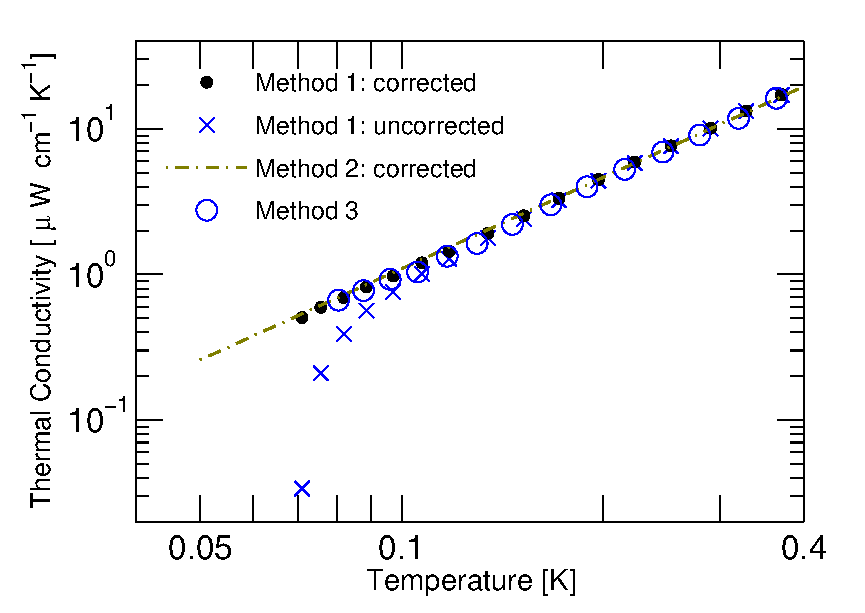
\includegraphics[width = 0.6\columnwidth]{Ti153_methods.eps}
\caption{{\small Plot of K(T) for Ti 15-3-3-3 foil showing Method 1 before and after compensating for constant parasitic powers. Results from Method 2 adjust for the same parasitic powers. (Color figure online)}}
\label{ti153_method}
\end{figure}

\begin{table}
\centering
\begin{threeparttable}
\begin{tabular}{lr}
\toprule
Sample & K(T) [uW/cm-K] \\
\midrule
2020 graphite & $7.88$ T$^{1.00}$ \\
V. SCP-5050 & $11.3$ T$^{1.99}$ \\
V. SCP-5000 & $13.8$ T$^{1.11}$ \\
V. SP-22 & $22.1$ T$^{2.15}$ \\
Ti 15-3-3-3 & $131.5$ T$^{2.08}$ \\
Graphlite & $160.0$ T$^{1.54}$ \\
Kapton-epoxy: & $10^{1.81 + 1.01log(T) - 0.348log^2(T)}$ \\
\bottomrule
\end{tabular}
\end{threeparttable}
\caption{{\small Parameterized K(T) measured for materials (Method 2). Only the Kapton-epoxy did not follow a power-law.}}
\label{cond_table}
\end{table}

\section{Thermal Conductivity Results}
Measured thermal conductivities are shown on the left plot of Figure \ref{plots}. Error bars are given for the points obtained using Method 1. The black error bars give the measurement uncertainty, while the green regions give the combined measurement and systematic uncertainty. In the same figure, we plot the curves produced from Method 2, given in Table \ref{cond_table}. We see exceptional agreement between the two measurement methods. Results from Method 3 are left out for readability. Overall errors in K(T) are estimated to be between 6\%-15\%, with the lowest temperature points being up to 20\%; these errors are dominated by uncertainty in power through the sample -- especially from parasitic heat loads at low temperatures -- and on uncertainty in defined sample length, due to the finite length of the thermometer mounts. Constant parasitic heat loads were typically $\sim 5$nW. These were calculated by measuring $\Delta T$ across the samples when no power was being applied; using the K(T) measured from Method 3, we then solved eqn 1 for $P_{parasitic}$.

The right side of Figure \ref{plots} compares our conductivity measurements to data in the literature. We see that the thermal conductivity of grade 2020 graphite is very similar to POCO AXM-5Q. In addition, both SCP-5000 and SCP-5050 have lower conductivity than their counterparts SP-1 and SP-22, making them very interesting for experimental applications. Our measured K(T) for Vespel SP-22 is lower than the results from J.R. Olson\cite{Olson1993}; this may be a real difference in K(T) due to material variation, or an error caused by uncertainty in parasitic heat loads. Our results for Graphlite were marginally higher than Runyan \& Jones' results\cite{Runyan2008}; this may be due to the fact that their group did not test official Graphlite, but a very similar CFRP with the same fiber fill volume and bisphenol-based epoxy \footnotemark \footnotetext{Information based on personal communication with the author.}.  The values obtained for Kapton-epoxy are consistent with the literature if we assume that the epoxy has higher K(T) than Kapton. For Ti 15-3-3-3, although our results are consistent at high temperatures with those reported by Wikus et al.\cite{Wikus2010}, we do not observe the sharp drop in conductivity they report below 500mK \footnotemark. \footnotetext{Wikus' sample became a superconductor at 3.89K. We expect that our material has these same properties, as it was processed from similar plate stock provided by TIMET.} We observe a similar drop in Figure \ref{ti153_method} for Method 1 when not accounting for parasitic heat loads, and believe that this may be the cause of the observed drop in their data. Nevertheless, Ti 15-3-3-3 exhibits a sufficiently low K(T) for use in cryogenic systems.

\section{Concluding Remarks}
This paper presented radiopurity and thermal conductivity data for materials with a low-background experiment in mind. The appropriate material for a given experiment will of course depend on the application. For electronic cabling, we have presented a low thermal conductivity Kapton-epoxy composite as a substrate and Ti 15-3-3-3 foil as trace material. For structural applications, materials such as Vespel (SP-1, SCP-5000, and SCP-5050), TIMET Ti 15-3-3-3, Graphlite CFRP, and purified AXM-5Q have demonstrated merit. Here, one must consider strength and stiffness requirements for the application, and thermal conductivity normalized to Young's modulus becomes a useful metric - a topic addressed in \cite{Runyan2008} and \cite{Kramer2013}. In these applications, mechanical properties set the amount of material needed, which in turn determines radioactivity (which scales by volume) and thermal conductance (which scales by g = A/L). As a practical consideration, price may factor into material choice. AXM-5Q, CFRP, and Ti 15-3-3-3 have comparably low prices, while Vespel products are significantly more expensive, with SCP-5000 and SCP-5050 being the most expensive (\$1,000 for a 1/4" $\oslash$ x 36" long rod at the time of this work). We have determined that for our purposes, Ti 15-3-3-3 and CFRP effectively combine low radioactivity, price, and thermal conductivity with high stiffness, and have selected them for use in the CDMS Experiment.

\begin{figure}[h]
\includegraphics[width = .984\textwidth,trim = 0 0 0 1.25cm]{K_plots_3.eps}
\caption{{\small Thermal conductivity of tested materials compared to other materials of interest. In the left plot, black error bars give measurement uncertainty, while the green shading gives systematic + measurement uncertainty at 60\% CL -- both are for the constant K(T) approximation method. In the left legend, $\parallel$ signifies that Graphlite was measured parallel to the fiber axis, and Kapton-epoxy/Ti 15-3-3-3 were measured parallel to the plane of the sheet. $\perp$ denotes that 2020 was measured perpendicular to the grain orientation. In both plots, the curves for our samples come from Table \ref{cond_table}. Other data is from: Graphlite\cite{Runyan2008}, Ti 15-3-3-3\cite{Wikus2010}, SP-22\cite{Olson1993}, SP-1\cite{Pobell1992}, AXM-5Q\cite{Woodcraft2009}. Kapton data is from a CDMS internal note by Dan Akerib (1995). (color version online)}}
\label{plots}
\end{figure}

\bigskip

\noindent \textbf{Acknowledgements}

\noindent The authors would like to thank Curbell Plastics and Tech-Etch for donating test samples. This work was funded by the Department of Energy and the National Science Foundation.

\begin{thebibliography}{99}

\bibitem{Hust1982}
J.G. Hust and A.B. Lankford, {\it Int. Journal of Thermophysics} \textbf{3}, 67, (1982).

\bibitem{Woodcraft2009}
A.L. Woodcraft et al., {\it Cryogenics} \textbf{49}, 159, (2009).

%, M. Barucci, P.R. Hastings, L. Lolli, V. Martelli, L. Risegari, and G. Ventura

\bibitem{Runyan2008}
M.C. Runyan and W.C. Jones, {\it Cryogenics} \textbf{48}, 448, (2008).

\bibitem{Wikus2010}
P. Wikus et al., {\it Cryogenics} \textbf{51}, 41, (2010).

%, S.A. Hertel, S.W. Leman, K.A. Mc{C}arthy, S.M. Ojeda, and E. Figueroa-{F}eliciano

\bibitem{Pobell1992}
F. Pobell, {\it Matter and Methods at Low Temperatures} (Springer--Verlag, Heidelberg, Germany, 1992).

\bibitem{Olson1993}
J.R. Olson, {\it Cryogenics} \textbf{33}, 729, (1993).

\bibitem{Didschuns2003}
I. Didschuns, A.L. Woodcraft, D. Bintley, and P.C. Hargrave, {\it Cryogenics} \textbf{44}, 293, (2003).

\bibitem{Kramer2013}
E. Kramer et al., "Material Selection for Cryogenic Support Structures". JOLT-1052

\bibitem{Akerib1995}
D. Akerib. Internal measurement for the CDMS Collaboration (1995).

\end{thebibliography}

\end{document}
